\documentclass[17pt]{beamer} %Makes presentation
%\documentclass[handout]{beamer} %Makes Handouts
\usetheme{Singapore} %Gray with fade at top
\useoutertheme[subsection=false]{miniframes} %Supppress subsection in header
\useinnertheme{rectangles} %Itemize/Enumerate boxes
\usecolortheme{seagull} %Color theme
\usecolortheme{rose} %Inner color theme

\definecolor{light-gray}{gray}{0.75}
\definecolor{dark-gray}{gray}{0.55}
\setbeamercolor{item}{fg=light-gray}
\setbeamercolor{enumerate item}{fg=dark-gray}

\setbeamertemplate{navigation symbols}{}
%\setbeamertemplate{mini frames}[default]
%\setbeamercovered{dynamics}
\setbeamerfont*{title}{size=\Large,series=\bfseries}
\setbeamerfont{footnote}{size=\tiny}

%\setbeameroption{notes on second screen} %Dual-Screen Notes
%\setbeameroption{show only notes} %Notes Output

\setbeamertemplate{frametitle}{\vspace{.5em}\bfseries\insertframetitle}
\newcommand{\heading}[1]{\noindent \textbf{#1}\\ \vspace{1em}}

\usepackage{bbding,color,multirow,times,ccaption,tabularx,graphicx,verbatim,booktabs}
\usepackage{colortbl} %Table overlays
\usepackage[english]{babel}
%\usepackage[latin1]{inputenc}
%\usepackage[T1]{fontenc}
\usepackage{lmodern}

%\author[]{Thomas J. Leeper}
\institute[]{
  \inst{}%
  Department of Government\\London School of Economics and Political Science
}

\usepackage{tikz}
\usetikzlibrary{shapes,arrows}
\usepackage[normalem]{ulem}
\usepackage{multicol}

\title{Translating Texts into Interpretations and Numbers}

% Primary and secondary source documents provide a written record of politically relevant events and processes. Texts can be used in a number of ways in political science research. How do we draw meaning from texts in qualitative and quantitative ways? How does textual information become useful data for making political inferences?



\date[]{}

\begin{document}

\frame{\titlepage}

\frame{\tableofcontents}

\frame{

\frametitle{Preview}

\begin{itemize}\itemsep1em
\item Two weeks on data collection
	\begin{itemize}
	\item Text analysis
	\item Interviewing methods
	\end{itemize}
\item Problem Set 3
	\begin{itemize}
	\item Due November 22
	\end{itemize}
\item Problem Set 4
	\begin{itemize}
	\item Discuss in class next 2 weeks
	\item Due December 13
	\end{itemize}
\end{itemize}

}

\section{Texts as Sources}
\frame{\tableofcontents[currentsection]}


\frame{

\frametitle{What counts as text?}

\begin{itemize}\itemsep1em
\item Primary sources
	\begin{itemize}
	\item Raw, original evidence
	\end{itemize}
\item Secondary sources
	\begin{itemize}
	\item Interpretations of raw evidence
	\end{itemize}
\item Tertiary sources
	\begin{itemize}
	\item Compendia or indices of two other types of sources
	\end{itemize}
\end{itemize}

}


\frame{

\frametitle{Use of Texts}

\begin{itemize}\itemsep1em
\item<1-> Text as description
	\begin{itemize}
	\item Rely on text in lieu of direct observation
	\item What do we gain? What do we lose?
	\end{itemize}
\item<2-> Text as DSOs
	\begin{itemize}
	\item Treat texts as units of analysis
	\item What do we gain? What do we lose?
	\end{itemize}
\end{itemize}


}

\frame{

\frametitle{Challenges of Text}

\begin{enumerate}\itemsep1em
\item Source ``Quality''
\item Subjectivity and differing perspectives
\item Historiography
\item Selection and confirmation bias
\end{enumerate}

\onslide<2->{But these are really the challenges of \textit{any} research!}

}


\frame{}

\section{Content Analysis}
\frame{\tableofcontents[currentsection]}

\frame{
\Large
\begin{center}
But the biggest issue is that once we have some texts, our interpretations are inherently subjective!
\end{center}
}


\frame{

Consider the following quote from a U.S. politician:

\begin{quote}
African Americans must stop making excuses and rely much more on themselves to get ahead in society.
\end{quote}

What does it mean? Is it positive or negative? Is it prejudicial?

}


\frame{
\begin{center}
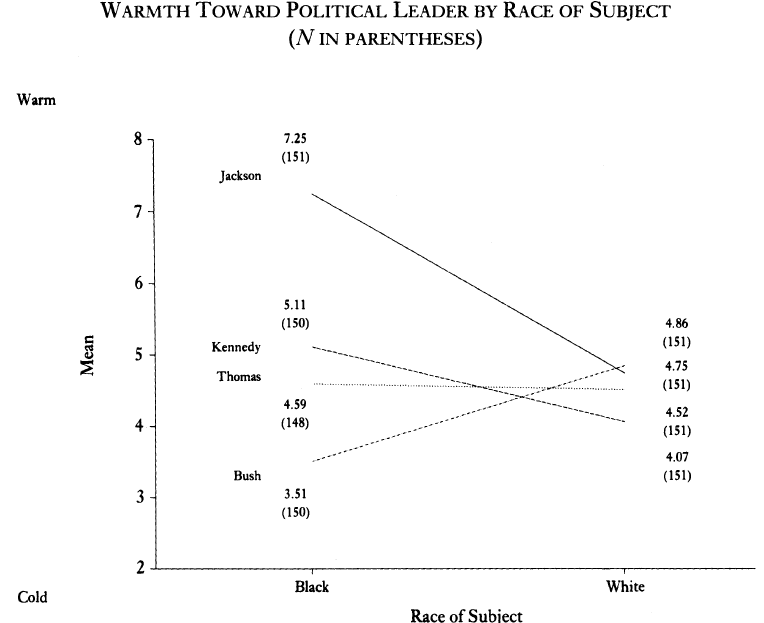
\includegraphics[height=0.8\textheight]{images/kuklinskihurley.png}
\end{center}

{\tiny
Kuklinski \& Hurley. 1994. ``On Hearing and Interpreting Political Messages: A Cautionary Tale of Citizen Cue-Taking.'' \textit{Journal of Politics} 56(3): 729--751.\\
}
}




\frame{

\frametitle{Content Analysis}

\begin{itemize}\itemsep0.5em
\item Definition: ``systematic description of the contents of a communication''
\item Treat texts as DSOs or a source of multiple DSOs
	\begin{itemize}
	\item Data set observation: score for a case on a variable
	\end{itemize}
\item Technique can be applied to any kind of document
\end{itemize}

}

% can be applied to any kind of document (primary, secondary, tertiary)
% need not be textual (we can content analyze images, videos, audio, actions/behaviors/expressions)
% graph showing textual input of one or more strings of text into an output of numbers/scores


\frame{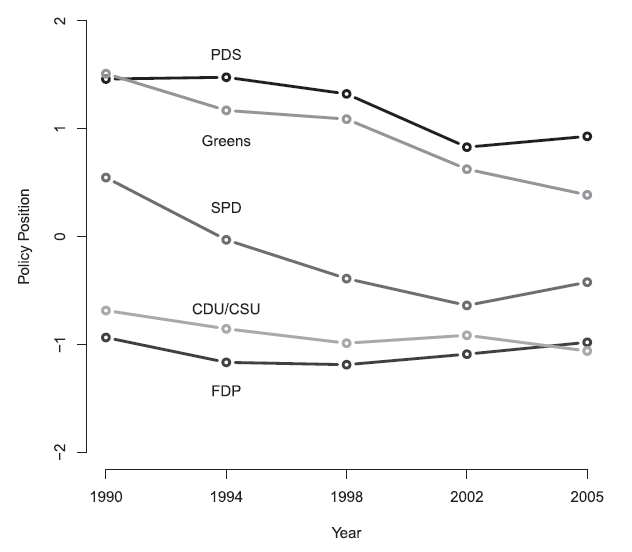
\includegraphics[height=\textheight]{images/grimmerstewart2.png}}
\frame{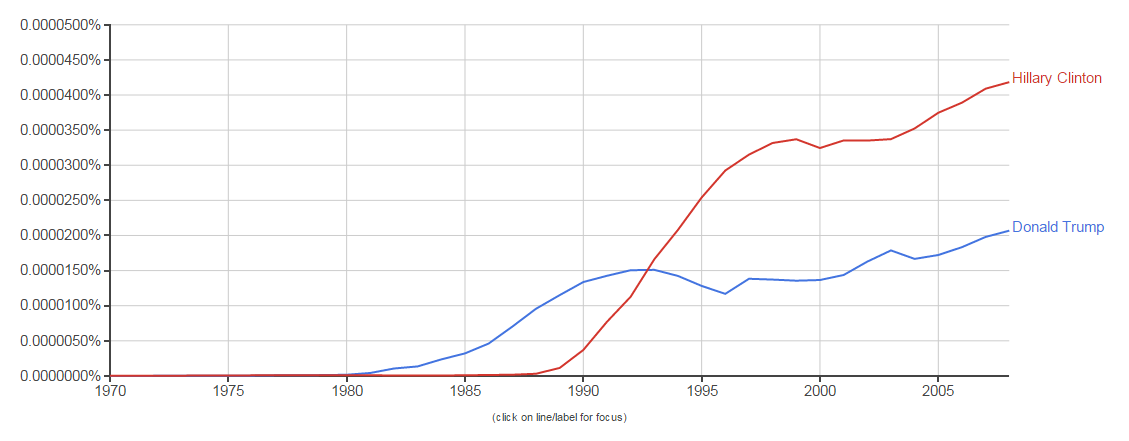
\includegraphics[width=\textwidth]{images/ngram1.png}}
\frame{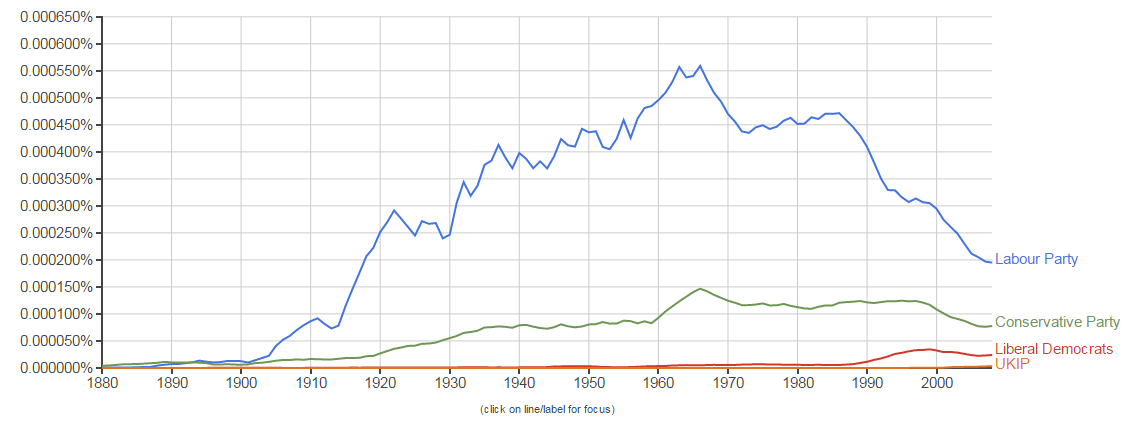
\includegraphics[width=\textwidth]{images/ngram2.png}}
\frame{\href{http://varianceexplained.org/r/trump-tweets/}{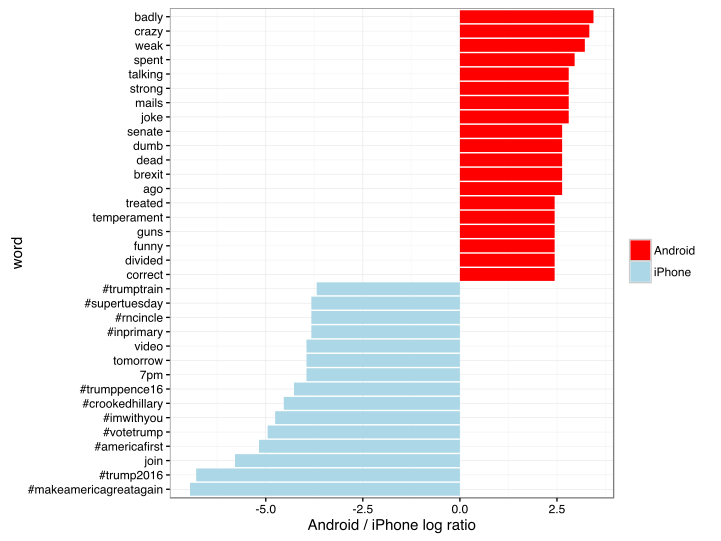
\includegraphics[width=\textwidth]{images/trumptweets.png}}}
\frame{\href{http://tidytextmining.com/tfidf.html}{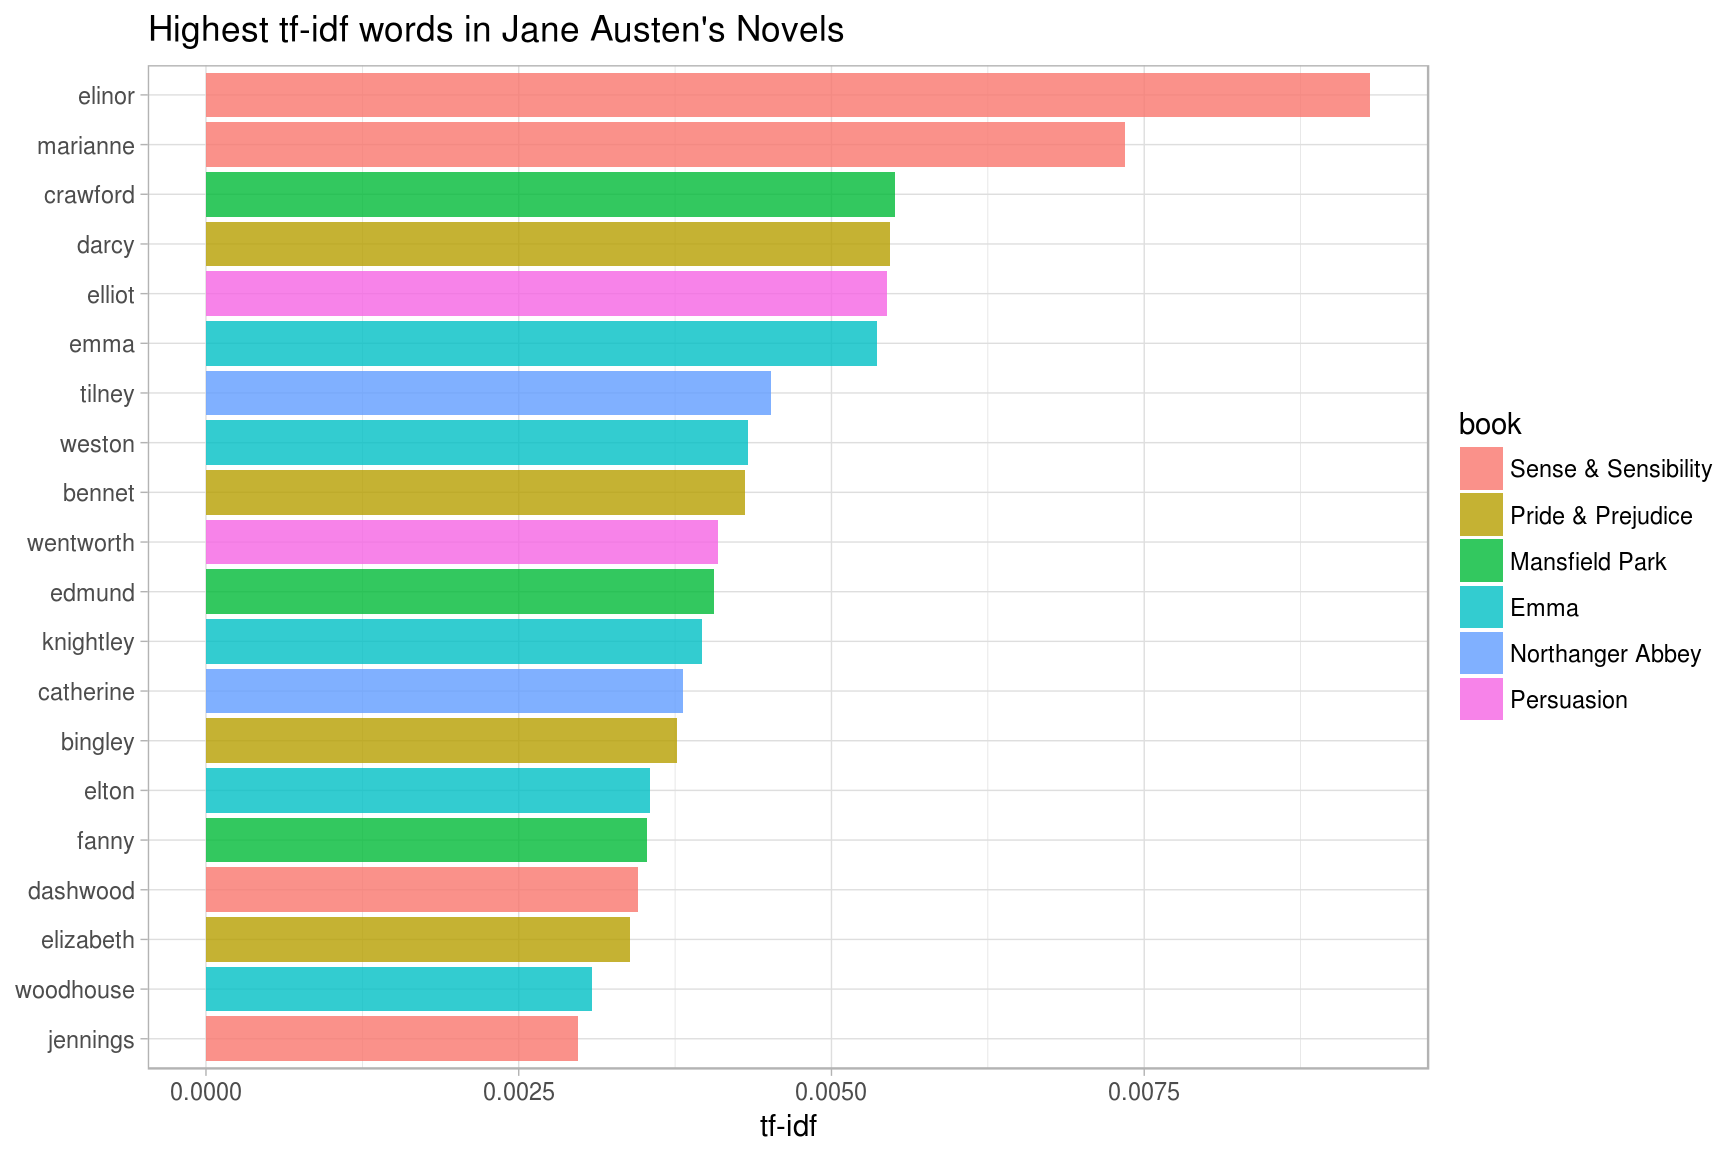
\includegraphics[width=\textwidth]{images/janeausten.png}}}


\frame{

\frametitle{Content Analysis Process}

\begin{enumerate}
\item<1-> Define a research question
\item<2-> Define concepts
\item<3-> Identify population (sample) of texts
\item<4-> Create a \textit{codebook} that describes how to operationalize concepts using text
\item<5-> Assign scores to text units based on codebook
\item<6-> Aggregate and summarize results
\end{enumerate}

}

% RQs and concepts are linked:
% what is the sentiment of this text?
% what is the ideology of this text?
% what ideas/arguments/frames/discourses are presented in this text?
% Tend to be descriptive RQs; causal inferences will come later once we've described the text fully
% content analysis is almost always comparative (comparing sources, authors, time period, contexts, etc.)

% what are the variables? what do we want to know about this text?

% scoring: ideology, positivity/negativity (both rely on word associations)
% dictionary methods (sentiment: lexicoder, ideology: wordfish)



\frame{

\frametitle{Example 1: Categorization}

\begin{itemize}\itemsep0.5em
\item Common RQ relates to categorization:\\ What is this text saying?
\item Example RQs:

	\begin{itemize}
	\item What arguments are raised in this text?
	\item Are certain ideas more prevalent in some texts than others?
	\item How is an issue discussed in politics?
	\end{itemize}

\item<2-> Running ex.: UKIP's 2015 Manifesto
\end{itemize}

}


\frame{

\frametitle{{\large Example 1 (Frames/Discourses)}}

If only all politicians could \textbf<2>{believe in Britain} as UKIP does. If only they could share our \textbf<2>{positive vision of Britain} as a \textbf<2>{proud}, \textbf<3-4>{independent sovereign nation}, a \textbf<4>{country respected on the world stage}, a \textbf<4>{major player in global trade}, with \textbf<4>{influence and authority} when it comes to tackling the pressing international issues of the day.


}
% categorization: 
% identification of frames, arguments, discourse

% discourses/frames
% 1: national pride/patriotism
% 2: independence
% 3: influential world power
% maybe others

% tabulating persons, issues, mentions
% necessarily iterative --> develop a set of categories as they are identified; requires revisiting texts


\frame{

\frametitle{{\large Example 2 (Mentions)}}


% persons
If only all \textbf<2>{politicians} could believe in \textbf<2>{Britain} as \textbf<2>{UKIP} does. If only they could share our positive vision of \textbf<2>{Britain} as a proud, independent sovereign nation, a country respected on the world stage, a major player in global trade, with influence and authority when it comes to tackling the pressing international issues of the day.
}


\frame{

\frametitle{{\large Example 3 (Issues/Priorities)}}

% issue mentions
\textcolor<2->{gray}{If only all politicians could believe in Britain as UKIP does.}
\textcolor<3->{gray}{If only they could share our positive vision of Britain}
\textcolor<4->{gray}{as a proud,} \textbf<4->{independent sovereign nation,}
\textcolor<5->{gray}{a country respected on the world stage,}
\textcolor<6->{gray}{a major player in} \textbf<6->{global trade}, 
\textcolor<7->{gray}{with influence and authority}
\textcolor<8->{gray}{when it comes to tackling the} \textbf<8>{pressing international issues} \textcolor<8->{gray}{of the day.}

}


\frame{

\frametitle{Developing Codebooks I}

\begin{itemize}
\item Developed \textit{deductively}\\
	\begin{enumerate}\itemsep0.5em
	\item Start with set of concepts
	\item Describe how those concepts might be expressed in text
	\item Create a ``coding scheme'' by which to score a case on a variable
	\end{enumerate}
\end{itemize}

}


\frame{

\frametitle{Developing Codebooks II}

\begin{itemize}
\item Developed \textit{inductively}\\
	\begin{enumerate}\itemsep0.5em
	\item Examine texts for key ideas and expressions
	\item Create a set of categories that summarize those expressions
	\item Examine new texts for expressions of those categories
	\item Expand and clarify the codebook as new concepts or expressions emerge
	\end{enumerate}
\end{itemize}

}



\frame{

\frametitle{Codebook Example I}

\footnotesize

\begin{enumerate}
\item<1-> Assign 1 if the text mentions ``Europe''
\item<2-> Count times ``Europe'' is mentioned
\item<3-> More complex example:
	\begin{itemize}
	\item Assign +1 if mentions ``Europe'' positively
	\item Assign -1 if mentions ``Europe'' negatively
	\item Assign 0 if text does not mention ``Europe''
	\end{itemize}
\item<4-> List all frames used in the text
\end{enumerate}

}

% different types of variables: binary, categorical/qualitative, interval (sums, proportions)



\begin{frame}

\frametitle{Example Scoring Sheet}

\normalsize

\begin{center}
\begin{tabular}{|l|r|r|r|r|} \hline
 & Mention & Count & Affect & Frame\\ \hline
UKIP &  &  & & \\ \hline
Conservative &  &  & & \\ \hline
Labour &  &  & & \\ \hline
LibDems &  &  & & \\ \hline
SNP &  &  & & \\ \hline
Greens &  &  & & \\ \hline
\end{tabular}
\end{center}

\end{frame}



\frame{

\frametitle{{\large Example 2: Dictionary Methods}}

\small

\begin{itemize}\itemsep0.5em
\item<1-> Rather than rely on subjective interpretation, dictionary methods create a ``dictionary'' of terms or expressions that operationalize a concept
\item<1-> Score is based on word presence of words or their frequencies
\item<1-> Often, goal is to categorize the text based on how it scores relative to other texts
	\begin{itemize}
	\item<2-> Sentiment (positivity/negativity)
	\item<2-> Ideology (left/right)
	\end{itemize}
\end{itemize}

}

% sentiment
\frame{

\frametitle{Affect/Sentiment}

If only all politicians could \textit<3->{believe} in Britain as UKIP does. If only they could \textit<3->{share} our \textbf<2->{positive} vision of Britain as a \textbf<2->{proud}, \textit<3->{independent} \textit<3->{sovereign} nation, a country \textbf<2->{respected} on the world stage, a \textit<3->{major} player in global trade, with \textbf<3->{influence} and \textit<3->{authority} when it comes to tackling the pressing international issues of the day.

}

% can create a dictionary for many ideas



\frame{

\frametitle{{\large Unit of Analysis}}

It can be difficult to decide what the correct unit of analysis is. Possibilities include:

\begin{multicols}{2}
\begin{itemize}\footnotesize\itemsep0em
\item Author/Source
\item Text as a whole
\item Section
\item Page
\item Paragraph
\item Sentence
\item Sentence fragment
\item Word
\end{itemize}
\end{multicols}

\only<2->{Smaller units can always be \textit{aggregated} later, but larger units cannot be \textit{disaggregated} later}

}

\begin{frame}

\frametitle{Example Scoring Sheet (Paragraph-level)}

\normalsize

\begin{center}
\begin{tabular}{|l|r|r|r|r|} \hline
 & Mention & Count & Affect & Frame\\ \hline
UKIP &  &  & & \\ \hline
Conservative &  &  & & \\ \hline
Labour &  &  & & \\ \hline
LibDems &  &  & & \\ \hline
SNP &  &  & & \\ \hline
Greens &  &  & & \\ \hline
\end{tabular}
\end{center}

\end{frame}


\begin{frame}

\frametitle{Example Scoring Sheet (Sentence-level)}

\normalsize

\begin{center}
\begin{tabular}{|l|r|r|r|r|} \hline
 & Sentence & Mention & Affect & Frame\\ \hline
UKIP & 1 &  &  & \\ \hline
UKIP & 2 &  &  & \\ \hline
UKIP & 3 &  &  & \\ \hline
UKIP & 4 &  &  & \\ \hline
UKIP & 5 &  &  & \\ \hline
\end{tabular}
\end{center}

\end{frame}


\frame{

\frametitle{Sentence}

\small

If only all politicians could believe in Britain as UKIP does.\\

\vspace{1em}

If only they could share our positive vision of Britain as a proud, independent sovereign nation, a country respected on the world stage, a major player in global trade, with influence and authority when it comes to tackling the pressing international issues of the day.

}

\frame{

\frametitle{Sentence fragments}

\small

If only all politicians could believe in Britain as UKIP does.\\

\vspace{0.5em}

If only they could share our positive vision of Britain \\

\vspace{0.5em}
as a proud, independent sovereign nation, \\

\vspace{0.5em}
a country respected on the world stage, \\

\vspace{0.5em}
a major player in global trade, \\

\vspace{0.5em}
with influence and authority \\

\vspace{0.5em}
when it comes to tackling the pressing international issues of the day.

}



% "bag of words" methods

\frame{

\frametitle{{\large ``Bag of Words'' Approaches I}}

\textcolor<2->{gray}{If} only all politicians could believe \textcolor<2->{gray}{in} Britain \textcolor<2->{gray}{as} UKIP does \textcolor<2->{gray}{.} \textcolor<2->{gray}{If} only they could share our positive vision \textcolor<2->{gray}{of} Britain \textcolor<2->{gray}{as} \textcolor<2->{gray}{a} proud\textcolor<2->{gray}{,} independent sovereign nation\textcolor<2->{gray}{,} \textcolor<2->{gray}{a} country respected \textcolor<2->{gray}{on} \textcolor<2->{gray}{the} world stage\textcolor<2->{gray}{,} \textcolor<2->{gray}{a} major player \textcolor<2->{gray}{in} global trade\textcolor<2->{gray}{,} \textcolor<2->{gray}{with} influence \textcolor<2->{gray}{and} authority \textcolor<2->{gray}{when} \textcolor<2->{gray}{it} comes \textcolor<2->{gray}{to} tackling \textcolor<2->{gray}{the} pressing international issues \textcolor<2->{gray}{of} \textcolor<2->{gray}{the} day\textcolor<2->{gray}{.}

}


\frame{

\frametitle{{\large ``Bag of Words'' Approaches II}}

only all politicians could believe Britain UKIP does only they could share our positive vision Britain proud independent sovereign nation country respected world stage major player global trade influence authority comes tackling pressing international issues day

}


\frame{

\frametitle{{\large ``Bag of Words'' Approaches III}}

\small

independent sovereign nation country international world global

\vspace{0.5em} 
positive proud respected major influence authority 

\vspace{0.5em} 
politicians player Britain Britain UKIP 

\vspace{0.5em} 
believe share tackling pressing 

\vspace{0.5em} 
could could does comes 

\vspace{0.5em} 
vision stage day trade issues 

\vspace{0.5em} 
only only all they our 

}

% term-document matrix


\frame{

\frametitle{N-grams and ``words''}

\small

\begin{itemize}\itemsep0.5em
\item<1-> ``Bag of words'' usually uses \textit{unigrams}
\item<2-> Unigrams are often ``stemmed''
	\begin{itemize}
	\item family, families, familiarity, and familial all become \textit{famil}.
	\end{itemize}
\item<3-> Can also be bigrams, trigrams, \textit{n}-grams
\item<4-> These allow for \textit{multi-word expressions}
	\begin{itemize}
	\item ``If only'' has a negative connotation even though ``if'' and ``only'' are basically neutral words on their own
	\end{itemize}
\end{itemize}


}


\section{Practicalities/Reflection}
\frame{\tableofcontents[currentsection]}


\frame{

\frametitle{{\large Content Analysis in Practice}}

\begin{itemize}\itemsep1em
\item Inductive processes generally require a ``training set'' and ``test set''
	\begin{itemize}
	\item Establish coding scheme on ``training set''
	\item Apply it to broader ``test set''
	\end{itemize}
\item<2-> Be cautious about scope conditions % codebook for news articles may not apply to speeches
\item<3-> Develop a precise and reliable codebook
\end{itemize}

}


\frame{

\frametitle{Intercoder Reliability}

\small

\begin{itemize}\itemsep0.75em
\item Definition: ``extent to which two (or more) coders agree on scores''
\item<2-> Have multiple coders analyze same text using coding scheme
\item<2-> Assess \% of time they assign same scores
\item<2-> Increase specificity of codebook if reliability is low (less than 80\%)
\end{itemize}

}


\frame{

\frametitle{{\large Manual versus Automated Techniques}}

\begin{itemize}\itemsep0.5em
\item Text analysis methods vary along a continuum from fully manual to fully automated
\item<2-> Automated methods can be computationally intensive
\item<3-> Automated methods make assumptions, but so do manual methods
\end{itemize}

}

% Why would we prefer manual versus automated methods?
% Are automated methods objective?

\frame{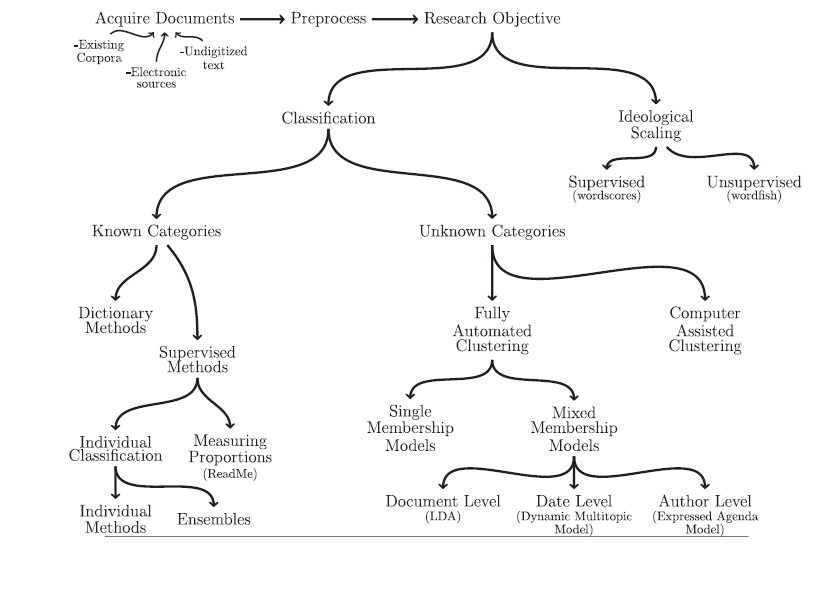
\includegraphics[width=\textwidth]{images/grimmerstewart.png}}


\frame{}

\frame{

\frametitle{``Quant'' or ``Qual''?}

Given what you know now, in what ways is content analysis a ``qualitative'' versus ``quantitative'' research method?

}


\frame{

\frametitle{Hands-On Practice}

\begin{itemize}\itemsep0.5em
\item There is no explicit lab for this topic
\item If you are interested, consider reading the Recommended text for this week, which includes hands-on exercises in R: \url{http://tidytextmining.com/}
\end{itemize}
}




\appendix
\frame{}

\end{document}
